\chapter{Introduction}

%--------------------------------------------------------------------------------------------------------
\section{Motivation}

Humans spend nearly one-third of their lives sleeping, highlighting its essential role in maintaining physical and cognitive well-being. Sleep is fundamental for brain development, memory consolidation, emotional regulation, and immune system function. However, disruptions in sleep quality and duration have been linked to various health issues, including cardiovascular diseases, obesity, diabetes, neurodegenerative disorders, and mental health conditions such as anxiety and depression \parencite{itani2017short}.\\

Despite its importance, sleep disorders are becoming increasingly prevalent, with conditions such as insomnia, sleep apnea, and narcolepsy affecting millions of individuals worldwide. It is estimated that around 50–70 million adults in the United States alone suffer from chronic sleep disorders, while an even larger population experiences occasional sleep disturbances. The growing burden of these disorders presents a significant public health concern, as inadequate sleep is associated with reduced productivity, impaired cognitive function, and increased healthcare costs \parencite{hirshkowitz2015national}.\\

Accurate sleep stage classification is a crucial step in diagnosing sleep disorders and understanding individual sleep patterns. Traditionally, sleep stage scoring relies on \ac{PSG} data, which requires trained specialists to manually annotate sleep stages based on recorded physiological signals. This manual process is labor-intensive, time-consuming, and subject to variability between scorers \parencite{yildirim2019deep}. To address these limitations, researchers have been actively exploring automated methods for sleep stage classification using machine learning and deep learning techniques \parencite{ardeshir2023sleep}.\\

To address the growing global burden of sleep disorders and the limitations of current diagnostic methods, there is a critical need for reliable, automated solutions that can support large-scale and long-term sleep monitoring. The motivation behind this study lies in the pursuit of more accessible, accurate, and scalable tools for sleep stage classification tools that can reduce the reliance on manual scoring and extend diagnostic capabilities beyond clinical settings. By leveraging recent advances in deep learning, particularly architectures capable of capturing intricate patterns in physiological data, this research aims to push the boundaries of automated sleep analysis. In doing so, it seeks to contribute meaningfully to early detection, personalized treatment, and improved outcomes for individuals affected by sleep-related conditions.
%--------------------------------------------------------------------------------------------------------
\section{Background}

\subsection{Foundations of Sleep Monitoring}

Understanding sleep and its underlying mechanisms requires a multidisciplinary perspective, drawing from neuroscience, electrophysiology, and biomedical engineering. The process of monitoring sleep is deeply rooted in our understanding of brain anatomy, how neural signals are generated and transmitted, and how they can be recorded and interpreted using various physiological monitoring techniques. \\

The brain is the central organ of the human nervous system, responsible for regulating thought, emotion, sensory perception, and motor functions. Alongside the spinal cord, it forms the central nervous system (CNS), managing both voluntary and involuntary processes essential for survival and homeostasis. \\

As illustrated in Figure \ref{fig:brain_structure}, the brain consists of three major regions: the cerebrum, cerebellum, and brainstem, each playing a vital role in maintaining physiological stability \parencite{kandel2000principles}. The cerebrum, the largest part, handles higher-order functions such as reasoning, memory, sensory processing, and voluntary movement. Beneath it, the cerebellum fine-tunes motor activity and supports balance and coordination. The brainstem, connecting the brain to the spinal cord, controls autonomic functions like breathing and heart rate \parencite{purves2013principles}.

\begin{figure}[H]
    \centering
    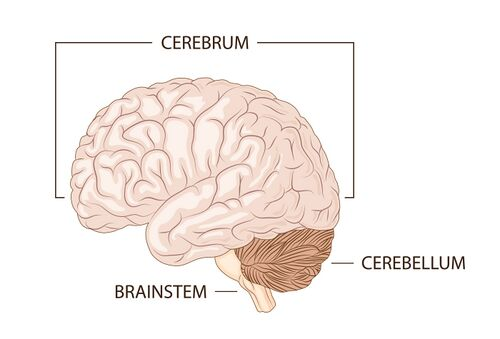
\includegraphics[width=0.55\linewidth]{Figures/Brain_anatomy.jpeg}
    \caption{Structural Organization of the Human Brain}
    \label{fig:brain_structure}
\end{figure}

The cerebral cortex, the brain’s outer layer, is shown in Figure \ref{fig:brain_2h_4l} and is divided into the left and right hemispheres. Each hemisphere contains four lobes frontal, parietal, temporal, and occipital each associated with specific cognitive and sensory roles. These anatomical divisions are especially relevant in sleep studies, as they contribute to distinct neural activities during different sleep stages.

\begin{figure}[H]
    \centering
    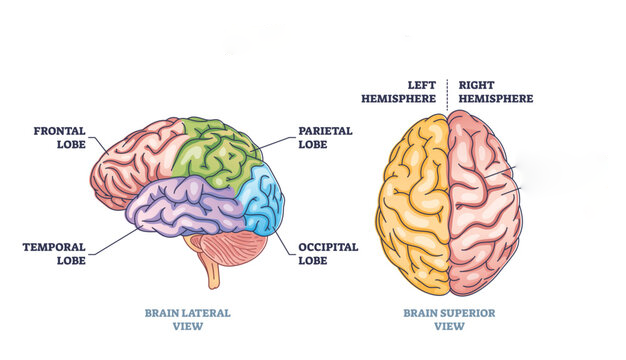
\includegraphics[width=0.6\linewidth]{Figures/brain 2h 4l.png}
    \caption{Structural division of the Brain into Lobes and Hemispheres}
    \label{fig:brain_2h_4l}
\end{figure}

Building upon the structural and functional overview of the brain, understanding how it generates and transmits signals is essential for interpreting the neural activity associated with sleep. Brain function relies on the communication between neurons specialized cells that transmit information via electrical and chemical signals. Neurons transmit information through action potentials, brief electrical impulses triggered by ion movement across the cell membrane. These signals travel along axons and activate neurotransmitter release at synapses, enabling communication across brain regions \parencite{bear2020neuroscience}. \\

To observe this activity, various techniques measure brain signals at different spatial and temporal resolutions. Among them, Electroencephalography (EEG) is particularly effective in sleep research, offering real-time insights into the brain’s electrical activity. EEG measures electrical activity from cortical neurons using electrodes placed on the scalp. These electrodes detect potential differences resulting from synchronized post-synaptic activity. As the raw signals are subtle, they are amplified and digitized for meaningful analysis \parencite{niedermeyer2005electroencephalography}. \\

\begin{figure}[H]
    \centering
    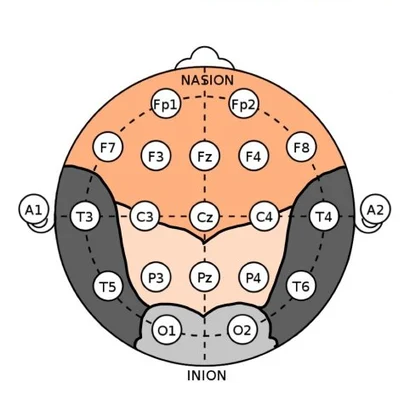
\includegraphics[width=0.65\linewidth]{Figures/the-10-20-system.png}
    \caption{The international 10-20 system for electrodes placement}
    \label{fig:the-10-20-system}
\end{figure}

To standardize data collection, EEG setups typically follow the 10–20 International System (Figure \ref{fig:the-10-20-system}), which positions electrodes based on skull landmarks. Electrodes are labeled by region F (frontal), C (central), P (parietal), O (occipital) with odd numbers for the left hemisphere, even for the right, and 'z' for midline placements. \\

While EEG provides focused insights into brain activity, comprehensive sleep analysis requires monitoring multiple physiological systems. Polysomnography (PSG) addresses this need by integrating various biophysical measurements, making it the gold standard for assessing sleep architecture and diagnosing sleep disorders. A standard PSG setup includes:
\begin{enumerate}
    \item \aclabelfont{EEG} (\acl{EEG}): Measures electrical activity in the brain.
    \item \aclabelfont{EOG} (\acl{EOG}): Detects eye movements.
    \item \aclabelfont{EMG} (\acl{EMG}): Monitors muscle activity.
    \item \aclabelfont{ECG} (\acl{ECG}): Tracks the electrical activity of the heart.
    \item \textbf{Respiratory Monitoring}: Includes sensors to monitor airflow, chest movements, and blood oxygen levels, offering insights into breathing patterns and respiratory health.
    \item \textbf{Other Parameters}: Depending on the specific application, \ac{PSG} may also include monitoring of additional factors such as temperature, blood pressure, or body movements.
\end{enumerate}

As illustrated in Figure \ref{fig:psg_electrodes}, PSG captures a synchronized view of brain and body function during sleep. This rich dataset enables accurate staging and the identification of abnormalities.
 
\begin{figure}[H]
    \centering
    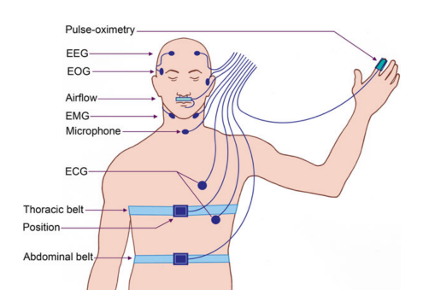
\includegraphics[width=0.65\linewidth]{Figures/psg.png}
    \caption{Electrode Placements for PSG Monitoring Across the Body}
    \label{fig:psg_electrodes}
\end{figure}
 
\subsection{Human Sleep}

Sleep is a fundamental biological process essential for maintaining overall health and cognitive function. It is a highly regulated state characterized by altered consciousness, reduced sensory perception, and diminished motor activity, allowing the body and brain to recover and process information. Contrary to being a passive state, sleep is an active and dynamic process involving complex physiological and neurological mechanisms. It plays a crucial role in cellular repair, immune system regulation, and metabolic homeostasis \parencite{walker2017we}.\\

Sleep is broadly classified into two main types: \ac{NREM} sleep and \ac{REM} sleep. These stages alternate cyclically throughout the night, forming sleep cycles that typically last between 90 and 120 minutes. A full night’s sleep consists of approximately four to six cycles, with the proportion of REM sleep increasing in later cycles, suggesting its critical role in cognitive processing and memory consolidation \parencite{carskadon2005normal}.\\

\ac{NREM} sleep accounts for approximately 75\%–80\% of total sleep and consists of three distinct stages. Stage 1 is a transitional phase between wakefulness and sleep, characterized by reduced muscle tone and slow eye movements. Stage 2 is marked by a decrease in body temperature and heart rate, with Sleep spindles and K-complexes observed in \ac{EEG} recordings, indicating the brain’s role in processing external stimuli and memory formation \parencite{de2003sleep}. Stage 3, also referred to as Deep sleep or Slow Wave Sleep, is the most restorative phase, playing a critical role in physical recovery, immune function, and long term memory consolidation \parencite{diekelmann2010memory}.\\

In contrast, REM sleep constitutes 20\%–25\% of total sleep and is characterized by rapid eye movements, vivid dreams, and heightened brain activity resembling wakefulness. This stage is essential for emotional regulation and cognitive functions such as problem-solving and creativity \parencite{bjorn2013sleep}. The dynamic alternation between NREM and REM sleep throughout the night reflects the brain's ongoing processes of neural reorganization and memory integration.\\

Brain wave activity during sleep varies across different stages, providing a reliable basis for identifying and classifying sleep phases. In the lighter stages of sleep, higher-frequency alpha and theta wavesdominate, signaling the brain’s gradual disengagement from external stimuli. These wave patterns are key indicators of early \ac{NREM} sleep. As sleep deepens, slow-wave delta activity becomes prominent, distinguishing Stage 3 sleep, which is essential for memory consolidation and tissue repair \parencite{sterpenich2007sleep}. During \ac{REM} sleep, a mixture of theta and beta waves emerges, resembling wakefulness and reflecting the brain's heightened activity associated with dreaming and cognitive processing \parencite{hobson2009rem}. By analyzing these characteristic neural oscillations, researchers can effectively classify sleep stages, aiding in the development of automated sleep staging models for clinical and research applications. Table \ref{tab:eeg_sleep_waves} presents the frequency bands of the characteristic wave types that occur during sleep.\\

\begin{table}[H]
    \centering
    \begin{tabular}{|c|c|}
        \hline
        \textbf{Wave Type} & \textbf{Frequency Range} \\ 
        \hline
        Slow-wave activity & 0.5–2 Hz \\ 
        \hline
        Delta waves & 0–3.99 Hz \\ 
        \hline
        Theta waves & 4–7.99 Hz \\ 
        \hline
        Alpha waves & 8–13 Hz \\ 
        \hline
        Beta waves & \textgreater 13 Hz \\ 
        \hline
    \end{tabular}
    \caption{EEG Frequency Bands Observed During Sleep}
    \label{tab:eeg_sleep_waves}
\end{table}

\subsection{Sleep Stages}

Human sleep, as discussed earlier, is a dynamic process consisting of distinct stages that cycle throughout the night. To systematically classify these stages, two widely recognized methodologies have been developed: the Rechtschaffen and Kales (R\&K) manual and the \ac{AASM} guidelines. While both methods aim to categorize sleep stages based on electrophysiological patterns, the R\&K system remains the most comprehensive and widely referenced framework due to its detailed classification and historical significance in sleep research \parencite{rechtschaffen1978techniques,iber2007aasm}.\\

The R\&K classification system, established in 1968, defines sleep architecture using \acs{EEG} (Electroencephalography), \acs{EOG} (Electrooculography), and \acs{EMG} (Electromyography) recordings. It divides sleep into five distinct stages:

\begin{enumerate}
    \item \textbf{NREM Stage 1}: This is the transition from wakefulness to sleep, lasting only a few minutes. It is characterized by low-amplitude, mixed-frequency brain waves (alpha and theta waves) \parencite{rechtschaffen1978techniques}. Slow rolling eye movements occur, and muscle activity decreases. The body begins to disengage from its surroundings in preparation for deeper sleep.

    \item \textbf{NREM Stage 2}: This stage makes up a significant portion of total sleep and is important for memory consolidation and sensory processing. It is marked by sleep spindles and K-complexes in \acs{EEG} recordings \parencite{de2003sleep}. These patterns help maintain sleep stability by reducing sensitivity to external disturbances. Muscle tone decreases, and body temperature drops as the body prepares for deeper sleep.

    \item \textbf{NREM Stage 3}: This stage is the first phase of deep sleep, with 20\%–50\% delta wave activity in \acs{EEG} recordings. It is essential for physical restoration, immune function, and hormone release \parencite{diekelmann2010memory}. Brain activity slows significantly, and waking up from this stage is difficult. Muscle activity is further reduced, and external stimuli have little effect.

    \item \textbf{NREM Stage 4}: This is the deepest sleep stage, with more than 50\% delta wave activity \parencite{diekelmann2010memory}. It plays a crucial role in cell repair, energy restoration, and memory consolidation. Waking up from this stage is very difficult, and disruptions can cause grogginess and cognitive impairment. This stage is vital for overall health, supporting growth, immune function, and metabolism.
    
    \item \textbf{REM}: This stage differs from \acs{NREM} sleep due to its unique brain activity, which resembles wakefulness. It features rapid eye movements and muscle atonia, which prevents movement during dreams \parencite{hobson2009rem}. \acs{REM} sleep is linked to cognitive functions such as emotional regulation, memory integration, and creative thinking \parencite{bjorn2013sleep}. Its proportion increases in later sleep cycles, highlighting its importance in overall sleep quality.
    
\end{enumerate}

In 2007, the AASM introduced a new sleep staging system to improve the R\&K method, particularly in distinguishing between \acs{NREM} stages, especially Stage 3 and Stage 4. The R\&K system is still used in some research due to its historical importance and consistency in comparing data from older studies. Despite the improvements made by the \acs{AASM} system, R\&K continues to be valuable for long-term research. Table \ref{tab:sleep_staging} below compares the sleep stages between the R\&K and \acs{AASM} methods.

\begin{table}[H]
    \centering
    \begin{tabular}{|l|c|}
        \hline
        \textbf{R\&K} & \textbf{AASM} \\
        \hline
         Wake Stage &  Wake Stage \\
        \hline
        \textbf{N-REM} Stage 1 & N1 Stage \\
        \hline
        \textbf{N-REM} Stage 2 & N2 Stage \\
        \hline
        \textbf{N-REM} Stage 3 & \multirow{2}{*}{N3 Stage} \\
        \cline{1-1}
        \textbf{N-REM} Stage 4 &  \\
        \hline
         REM Stage &  REM Stage \\
        \hline
    \end{tabular}
    \caption{Comparison of R\&K and AASM Sleep Staging Levels}
    \label{tab:sleep_staging}
\end{table}

%--------------------------------------------------------------------------------------------------------
\section{Problem Statement}

Deep learning has shown great potential in automating sleep stage classification. However, many existing models process Polysomnography (PSG) signals as raw time-series data, which may not fully capture the spatial, temporal, and spectral dependencies inherent in these signals. To address this limitation, researchers have recently explored transforming \ac{PSG} data into image like representations such as spectrograms or time-series-to-image conversions, allowing the use of advanced computer vision models to enhance classification performance.\\

Despite these advancements, traditional \acp{CNN}, which are commonly used in sleep research, often struggle to capture long-range dependencies in \ac{PSG} data. Additionally, generalization remains a significant challenge, as sleep patterns vary widely between individuals due to factors such as age, lifestyle, and underlying health conditions. Therefore, there is a pressing need for more advanced techniques capable of effectively capturing spatial, temporal, and spectral dependencies while also being robust to subject-to-subject variability.\\

This research aims to address these challenges by leveraging \acp{ViT} for sleep stage classification using \ac{PSG} derived image representations. Unlike \acp{CNN}, \acp{ViT} utilize self-attention mechanisms to model both local and global dependencies, making them well-suited for complex sleep data. By applying \acp{ViT}, this study seeks to improve classification accuracy, uncover meaningful patterns related to sleep disorders, and enhance model adaptability to individual differences, ultimately advancing the reliability of automated sleep stage classification.

%--------------------------------------------------------------------------------------------------------
\section{Research Objectives}
The primary objective of this research is to develop an accurate Vision Transformers (ViTs) based model for automatic sleep stage classification using Polysomnography (PSG) data. PSG signals are continuous, time-dependent recordings that capture various physiological activities during sleep, such as brain activity (EEG), eye movements (EOG), muscle tone (EMG), and other biosignals. Due to their temporal nature, PSG signals resemble time series data, where variations over time provide critical insights into different stages of sleep. To effectively leverage ViTs, this study focuses on optimizing the transformation of PSG signals into informative image representations while also ensuring model interpretability for reliable and transparent sleep stage prediction. Other specific objectives are as follows:
\begin{enumerate}
    \item Investigate different image transformation techniques for \ac{PSG} signals.
    \item Identify the most effective frequency representations for \ac{PSG} based image transformations.
    \item Identify \ac{GAN} based methods for data augmentation to improve model performance.
\end{enumerate}
%--------------------------------------------------------------------------------------------------------
\section{Significance of the Study }

Accurate and reliable sleep stage classification plays a crucial role in the diagnosis and treatment of sleep disorders, which affect a significant portion of the global population. Traditional approaches to sleep stage classification, often reliant on manual scoring of Polysomnographic (PSG) recordings by trained experts, are time-consuming, prone to inter-scorer variability, and not scalable in clinical settings. While automated methods using classical machine learning and early deep learning models have demonstrated potential, they frequently suffer from limitations such as reliance on handcrafted features, difficulty in capturing long-range dependencies in physiological signals, and poor generalization to real-world clinical data. \\

This research addresses these challenges by leveraging recent advances in deep learning specifically, Vision Transformers (ViTs) to develop a novel framework for automatic sleep stage classification. By transforming Electroencephalography (EEG) signals into time-frequency image representations such as spectrograms, Gramian Angular Fields (GAF), and Markov Transition Fields (MTF), the study enables the use of powerful computer vision models trained on large scale datasets to extract deep semantic features from physiological data. Furthermore, the application of Generative Adversarial Networks (GANs) for targeted data augmentation helps to mitigate class imbalance, a persistent issue in sleep datasets where certain stages like S1 or Rapid Eye Movement (REM) stage are significantly underrepresented. \\

The significance of this work lies not only in advancing the technical methodology for sleep stage classification but also in demonstrating the potential of combining modern vision-based architectures with physiological signal processing. It contributes to the growing body of research advocating for cross domain innovations in biomedical applications and paves the way for more accurate, scalable, and generalizable tools for sleep medicine. Additionally, by highlighting research gaps such as the limited use of pre-trained ViTs and GAN augmented transformer models, this study sets the stage for future explorations into transformer-based frameworks for a wide range of medical time-series analysis tasks.

%--------------------------------------------------------------------------------------------------------
\section{Organization of the Thesis }

\textbf{Chapter 2:} Presents a comprehensive review of existing literature on sleep stage classification and covers traditional approaches to sleep stage classification, including machine learning and early deep learning methods, followed by the use of transformers in medical signal analysis. It explores transforming Polysomnography (PSG) signals into image representations using time-frequency techniques and methods like \ac{GAF} and \ac{MTF}, as well as the application of Generative Adversarial Networks (GANs) for data augmentation to address class imbalance. The chapter concludes by identifying research gaps, including the limited use of pre-trained Vision Transformers (ViTs) and GAN based augmentation for transformer models in sleep stage classification. \\

\textbf{Chapter 3:} Presents the theoretical foundations and experimental framework of this research. It covers key concepts such as time-series-to-image transformation methods, frequency downsampling techniques, Deep Convolutional GANs (DCGANs), and Vision Transformers (ViTs). The methodology section details signal preprocessing and six experiments evaluating image transformation techniques, sampling frequencies, ViT models, and GAN based augmentation, concluding with the final model selection process. \\

\textbf{Chapter 4:} Describes the datasets and data acquisition methods used in this research. \\

\textbf{Chapter 5:} Examines key aspects of the dataset before model training. It includes artifact detection to identify and address noise in Electroencephalography (EEG) signals and an analysis of inter-subject variations in EEG to understand differences across individuals. These analyses provide insights into data quality and variability, ensuring a robust foundation for subsequent experiments. \\

\textbf{Chapter 6:} Presents the findings from the experiments conducted in this study. It evaluates the performance of different image transformation techniques, the impact of sampling frequency and resampling methods, and the effectiveness of pre-trained versus from-scratch Vision Transformers. Additionally, it assesses various pre-trained ViT models, the training and tuning of DCGAN for synthetic image generation, and the impact of GAN augmented data. The chapter concludes with the selection of the final model. \\

\textbf{Chapter 7:} Summarizes the key findings of this research and their implications for sleep stage classification. The conclusion highlights the effectiveness of Vision Transformers and GAN based augmentation. The chapter also discusses potential directions for future research, including improving data augmentation techniques, exploring alternative transformer architectures, and enhancing model generalization across diverse datasets.

